\subsection{WAL-E}
\textbf{Ссылка}: \href{https://github.com/heroku/WAL-E}{github.com/heroku/WAL-E}

WAL-E предназначенная для непрерывной архивации PostgreSQL WAL-logs в S3 и управления использованием pg\_start\_backup и pg\_stop\_backup. Утилита написана на Python и разработана в компании \href{http://www.heroku.com/}{Heroku}, где её активно используют. 

\subsubsection{Установка}

У WAL-E есть пару зависимостей: lzop, psql, mbuffer, python 2.6+ и несколько python библиотек (gevent >= 0.13, boto >= 2.0). Также для удобства настроек переменных среды устанавливается daemontools. На Ubuntu это можно все поставить одной командой:

\begin{lstlisting}[label=lst:wal-e1,caption=Установка зависимостей для WAL-E]
# PostgreSQL уже установлен
aptitude install git-core python-dev python-setuptools build-essential libevent-dev lzop mbuffer daemontools daemontools-run
\end{lstlisting}

Теперь установим WAL-E:

\begin{lstlisting}[label=lst:wal-e2,caption=Установка WAL-E]
git clone git://github.com/heroku/WAL-E.git
cd WAL-E
python setup.py build
sudo python setup.py install
\end{lstlisting}

После успешной установки можно начать работать с WAL-E. 

\subsubsection{Работа}
Как уже писалось, WAL-E сливает все данные в AWS S3, поэтому нам потребуются <<Access Key ID>> и <<Secret Access Key>>. Команда для загрузки бэкапа всей базу данный в S3:

\begin{lstlisting}[label=lst:wal-e3,caption=Загрузка бэкапа всей базы данных в S3]
AWS_SECRET_ACCESS_KEY=... wal-e                     \
  -k AWS_ACCESS_KEY_ID                                \
  --s3-prefix=s3://some-bucket/directory/or/whatever  \
  backup-push /var/lib/postgresql/9.2/main
\end{lstlisting}

Где <<s3-prefix>>~--- урл, который содержит имя S3 бакета (bucket) и путь к папке, куда следует складывать бэкапы. Команда для загрузки WAL-логов на S3:

\begin{lstlisting}[label=lst:wal-e4,caption=Загрузка WAL-логов на S3]
AWS_SECRET_ACCESS_KEY=... wal-e                     \
  -k AWS_ACCESS_KEY_ID                                \
  --s3-prefix=s3://some-bucket/directory/or/whatever  \
  wal-push /var/lib/postgresql/9.2/main/pg_xlog/WAL_SEGMENT_LONG_HEX
\end{lstlisting}

Для управления этими переменными окружения можно использовать команду envdir (идет в поставке с daemontools). Для этого создадим envdir каталог:

\begin{lstlisting}[label=lst:wal-e5,caption=WAL-E с envdir]
$ mkdir -p /etc/wal-e.d/env
$ echo "secret-key" > /etc/wal-e.d/env/AWS_SECRET_ACCESS_KEY
$ echo "access-key" > /etc/wal-e.d/env/AWS_ACCESS_KEY_ID
$ echo 's3://some-bucket/directory/or/whatever' > /etc/wal-e.d/env/WALE_S3_PREFIX
$ chown -R root:postgres /etc/wal-e.d
\end{lstlisting}

После создания данного каталога возможно появляется возможность запускать WAL-E команды гораздо проще и с меньшим риском случайного использования некорректных значений:

\begin{lstlisting}[label=lst:wal-e6,caption=WAL-E с envdir]
$ envdir /etc/wal-e.d/env wal-e backup-push ...
$ envdir /etc/wal-e.d/env wal-e wal-push ...
\end{lstlisting}

Теперь настроим PostgreSQL для сбрасывания WAL-логов в S3 c помощью WAL-E. Отредактируем postgresql.conf:

\begin{lstlisting}[label=lst:wal-e7,caption=Настройка PostgreSQL]
wal_level = hot_standby # или archive, если PostgreSQL < 9.0
archive_mode = on
archive_command = 'envdir /etc/wal-e.d/env /usr/local/bin/wal-e wal-push %p'
archive_timeout = 60
\end{lstlisting}

Лучше указать полный путь к WAL-E (можно узнать командой <<which wal-e>>), поскольку PostgreSQL может его не найти. После этого нужно перегрузить PostgreSQL. В логах базы вы должны увидить что то подобно:

\begin{lstlisting}[label=lst:wal-e8,caption=Логи PostgreSQL]
2012-11-07 14:52:19 UTC LOG:  database system was shut down at 2012-11-07 14:51:40 UTC
2012-11-07 14:52:19 UTC LOG:  database system is ready to accept connections
2012-11-07 14:52:19 UTC LOG:  autovacuum launcher started
2012-11-07T14:52:19.784+00 pid=7653 wal_e.worker.s3_worker INFO     MSG: begin archiving a file
        DETAIL: Uploading "pg_xlog/000000010000000000000001" to "s3://cleverdb-pg-backups/pg/wal_005/000000010000000000000001.lzo".
2012-11-07 14:52:19 UTC LOG:  incomplete startup packet
2012-11-07T14:52:28.234+00 pid=7653 wal_e.worker.s3_worker INFO     MSG: completed archiving to a file 
        DETAIL: Archiving to "s3://cleverdb-pg-backups/pg/wal_005/000000010000000000000001.lzo" complete at 21583.3KiB/s. 
2012-11-07T14:52:28.341+00 pid=7697 wal_e.worker.s3_worker INFO     MSG: begin archiving a file
        DETAIL: Uploading "pg_xlog/000000010000000000000002.00000020.backup" to "s3://cleverdb-pg-backups/pg/wal_005/000000010000000000000002.00000020.backup.lzo".
2012-11-07T14:52:34.027+00 pid=7697 wal_e.worker.s3_worker INFO     MSG: completed archiving to a file 
        DETAIL: Archiving to "s3://cleverdb-pg-backups/pg/wal_005/000000010000000000000002.00000020.backup.lzo" complete at 00KiB/s. 
2012-11-07T14:52:34.187+00 pid=7711 wal_e.worker.s3_worker INFO     MSG: begin archiving a file
        DETAIL: Uploading "pg_xlog/000000010000000000000002" to "s3://cleverdb-pg-backups/pg/wal_005/000000010000000000000002.lzo".
2012-11-07T14:52:40.232+00 pid=7711 wal_e.worker.s3_worker INFO     MSG: completed archiving to a file 
        DETAIL: Archiving to "s3://cleverdb-pg-backups/pg/wal_005/000000010000000000000002.lzo" complete at 2466.67KiB/s. 
\end{lstlisting}

Если похожего не видно в логах, тогда нужно смотреть что за ошибка появляется и исправлять её.

Для того, что бы бэкапить всю базу достаточно выполнить данную команду:

\begin{lstlisting}[label=lst:wal-e9,caption=Загрузка бэкапа всей базы данных в S3]
$ envdir /etc/wal-e.d/env wal-e backup-push /var/lib/postgresql/9.2/main
2012-11-07T14:49:26.174+00 pid=7493 wal_e.operator.s3_operator INFO     MSG: start upload postgres version metadata
        DETAIL: Uploading to s3://cleverdb-pg-backups/pg/basebackups_005/base_000000010000000000000006_00000032/extended_version.txt.
2012-11-07T14:49:32.783+00 pid=7493 wal_e.operator.s3_operator INFO     MSG: postgres version metadata upload complete
2012-11-07T14:49:32.859+00 pid=7493 wal_e.worker.s3_worker INFO     MSG: beginning volume compression
        DETAIL: Building volume 0.
...
HINT:  Check that your archive_command is executing properly.  pg_stop_backup can be canceled safely, but the database backup will not be usable without all the WAL segments.
NOTICE:  pg_stop_backup complete, all required WAL segments have been archived
\end{lstlisting}

\begin{figure}[h!]
  \center{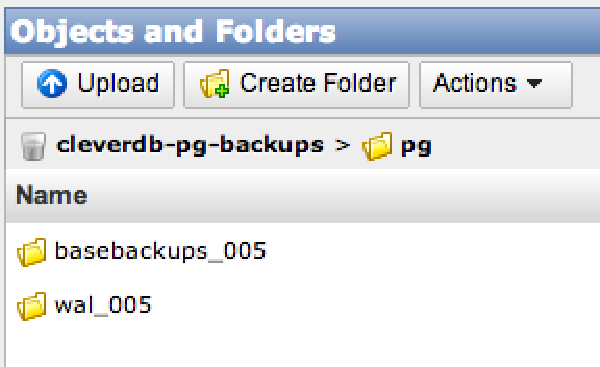
\includegraphics[width=0.6\textwidth]{wale1.pdf}}
  \caption{Папка бэкапов на S3}
  \label{fig:wal-e1}
\end{figure}

\begin{figure}[h!]
  \center{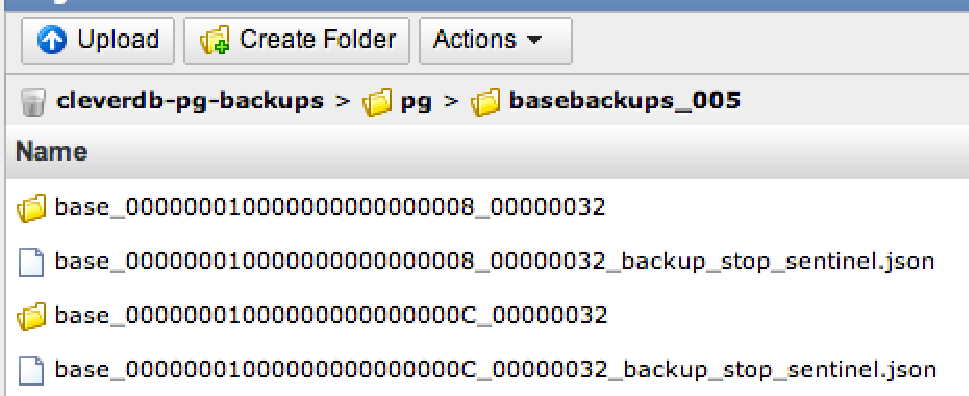
\includegraphics[width=0.6\textwidth]{wale2.pdf}}
  \caption{Папка бэкапов базы на S3}
  \label{fig:wal-e2}
\end{figure}

\begin{figure}[h!]
  \center{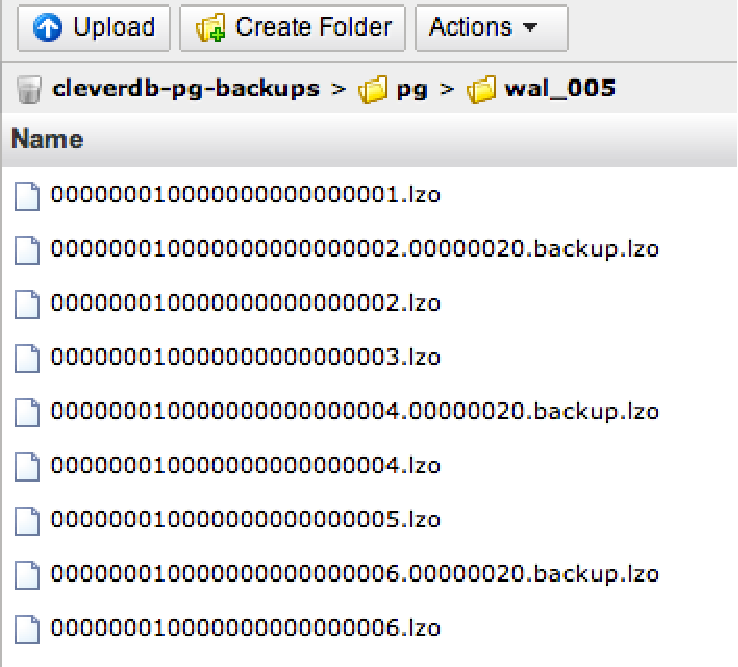
\includegraphics[width=0.6\textwidth]{wale3.pdf}}
  \caption{Папка WAL-логов на S3}
  \label{fig:wal-e3}
\end{figure}

Данный бэкап лучше делать раз в сутки (например, добавить в crontab). На рис~\ref{fig:wal-e1}-\ref{fig:wal-e3} видно как хранятся бэкапы на S3. Бэкапы сжаты через lzop\footnote{http://en.wikipedia.org/wiki/Lzop}. Данный алгоритм хуже сжимает, чем gzip, но скорость сжатия намного быстрее (приблизительно 25Мб/сек используя 5\% ЦПУ). Чтобы уменьшить нагрузку на чтения с жесткого диска бэкапы отправляются через mbuffer (опцией <<cluster-read-rate-limit>> можно ограничить скорость чтения, если это требуется).

Теперь перейдем к восстановлению данных. Для восстановления базы из бэкапа использутеся <<backup-fetch>> команда:

\begin{lstlisting}[label=lst:wal-e10,caption=Восстановление бэкапа базы из S3]
$ sudo -u postgres bash -c "envdir /etc/wal-e.d/env wal-e  --s3-prefix=s3://some-bucket/directory/or/whatever backup-fetch /var/lib/postgresql/9.2/main LATEST"
\end{lstlisting}

Где <<LATEST>> означает восстановится из последнего актуального бэкапа (PostgreSQL в это время должен быть остановлен). Для восстановления из более позднего бэкапа:

\begin{lstlisting}[label=lst:wal-e11,caption=Восстановление старшего бэкапа из S3]
$ sudo -u postgres bash -c "envdir /etc/wal-e.d/env wal-e  --s3-prefix=s3://some-bucket/directory/or/whatever backup-fetch /var/lib/postgresql/9.2/main base_LONGWALNUMBER_POSITION_NUMBER"
\end{lstlisting}

Для получения списка доступных бэкапов есть команда <<backup-list>>:

\begin{lstlisting}[label=lst:wal-e12,caption=Список бэкапов]
$ envdir /etc/wal-e.d/env wal-e backup-list
name	last_modified	expanded_size_bytes	wal_segment_backup_start	wal_segment_offset_backup_start	wal_segment_backup_stop	wal_segment_offset_backup_stop
base_000000010000000000000008_00000032	2012-11-07T14:53:47.000Z		000000010000000000000008	00000032		
base_00000001000000000000000C_00000032	2012-11-07T15:00:08.000Z		00000001000000000000000C	00000032
\end{lstlisting}

После завершения работы с основным бэкапом для полного восстановления нужно считать WAL-логи (чтобы данные обновились до последнего состояния) и для этого используем recovery.conf:

\begin{lstlisting}[label=lst:wal-e13,caption=recovery.conf]
restore_command = 'envdir /etc/wal-e.d/env /usr/local/bin/wal-e wal-fetch "%f" "%p"'
\end{lstlisting}

После создания этого файла нужно запустить PostgreSQL. Через небольшой интервал времени база станет полностью восстановленной. 

Для удаления старых бэкапов (или вообще всех) используется команда <<delete>>:

\begin{lstlisting}[label=lst:wal-e14,caption=Удаление бэкапов]
# удаления старых бэкапов старше base_00000004000002DF000000A6_03626144
$ envdir /etc/wal-e.d/env wal-e delete --confirm before base_00000004000002DF000000A6_03626144
# удаления всех бэкапов
$ envdir /etc/wal-e.d/env wal-e delete --confirm everything
\end{lstlisting}

Без опции <<confirm>> команды будут запускатся и показывать, что будет удаляться, но фактического удаления не будет производится (dry run).

\subsubsection{Заключение}
WAL-E 